\chapter{Results}

\todo{Model evaluation and validation}
\todo{- Explain the final model paramters, explain}
\todo{- Explain the and show the loss funstion, show the confision matrix}
\todo{justification}
\todo{- Compare the final results to the bench mark - compare the confustion matrix to the once we have on the paper, also compare to the graph the score value, explain and show the problem is adiculately solved}


\section{Confusion Matrix}
At this point, we have a trained model with optimized parameters. In order for the model to be evaluated, we compute the confusion matrix $C$ is also known as error matrix. This matrix allows us to visualize of the performance of the algorithm. Each column of the matrix represents the instances in a predicted class while each row represents the instances in an actual class. This matrix shows the True Positive (TP), False Negative (FN), False Positive (FP) and True Negative (TN). The diagonal elements of the matrix represent the number of points for which the predicted label is equal to the true label, while off-diagonal elements are those that are mislabeled by the classifier. Figure \ref{fig:confusionbad} show the normalized confusion matrix for a MLP network which is not optimized yet. This kind of normalization can be interesting in case of class imbalance to have a more visual interpretation of which class is being misclassified. Labels are: PC (Planetary Candidates), NTP (None Transiting Phenomena),  AFP (Astrophysical False Positive) 

\begin{figure}[!h]
\begin{center}
        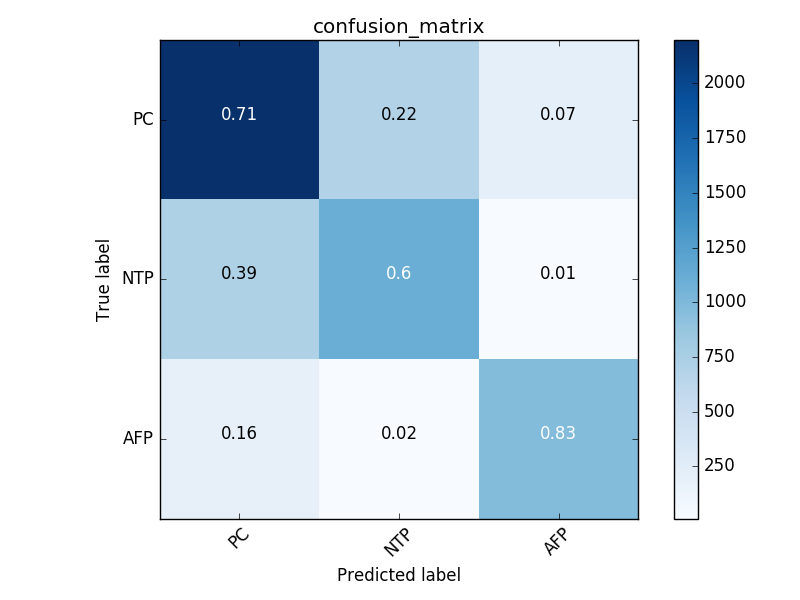
\includegraphics[width=0.5\textheight]{img/confusion_matrix_bad.png}
        \caption{Normalized Confusion Matrix. Unoptimized network predictions . Model Parameters are: \texttt{activation = identity, learning\_rate\_init\_num = 0.2, momentum\_num = 0}}  \label{fig:confusionbad}
\end{center}
\end{figure}

I also compute the accuracy (score) of the predictions.  In multilabel classification, the function returns the subset accuracy. If the entire set of predicted labels for a sample strictly match with the true set of labels, then he subset accuracy is 1.0; otherwise, it is 0.0. The accuracy is computed using equation \ref{eq:score}. For the example shown in the figure \ref{fig:confusionbad} has the accuracy score of $0.687$.

\begin{equation}
accuracy(y, \hat{y}) = \frac{1}{n_{samples}}\sum_{i=0}^{n_{samples}}I(\hat{y_i} = y_i)
\label{eq:score}
\end{equation}

where, $\hat{y}$t is the predicted value of the $i^{th}$ sample $y_i$ is the corresponding true value and $I(x)$ is the indicator function.

\begin{figure}[!h]
\begin{center}
        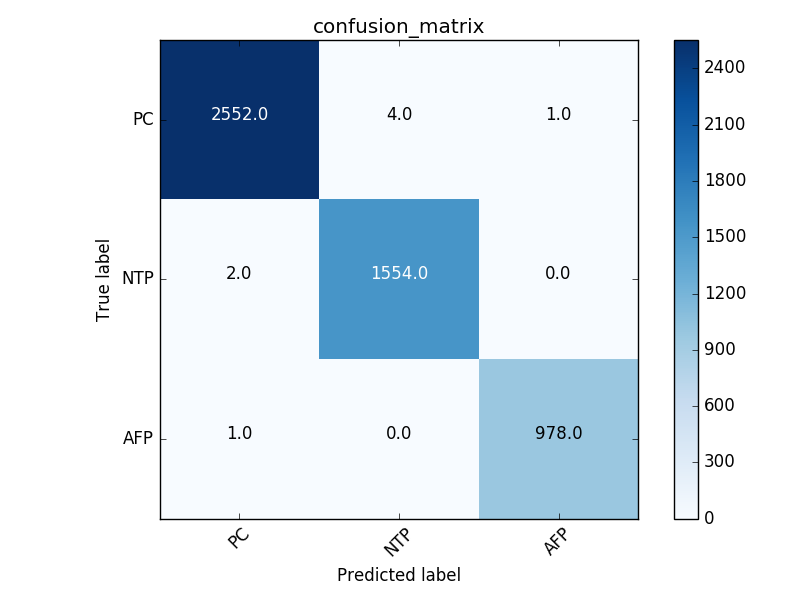
\includegraphics[width=0.5\textheight]{img/confusion_matrix_good.png}
        \caption{Optimized MLP network predictions.}  \label{fig:confusiongood}
\end{center}
\end{figure}


Finally, the confusion matrix that produced by the classifier that is properly tuned is shown in the figure \ref{fig:confusiongood}. I am showing the confusion matrix without normalizing it. The accuracy score that produces by this classifier is $0.998$. Due to high accuracy, the normalized matrix will have $1.0$ for the diagonal values and the $0.0$ for the off-diagonal values. It is clear the network is capable of classifying the Kepler Threshold Crossing Event Catalog with a high degree of accuracy. Glancing at the confusion matrix,  only 5 of the event are falsely labeled for the known planetary candidates (4 as NTP and 1 as an AFP). For the NTP its only 2 of the events are incorrectly classify as PCs and for the AFP there is only 1 one incorrect classification. 

Bench mark from the paper

